\documentclass[10pt]{beamer}

\usetheme[progressbar=frametitle, numbering=fraction,]{metropolis}

\usepackage{booktabs}
\usepackage{pgfplots}
\usepgfplotslibrary{dateplot}
\usepackage{texshade}      
\usepackage{amsmath}
\usepackage{amssymb}
\usepackage{xspace}
\usepackage{xcolor}
\usepackage{appendixnumberbeamer}
\usepackage{multirow}
\usepackage{verbatim}

\usepackage{tikz}
\usetikzlibrary{shapes.geometric, arrows}
\tikzstyle{startstop} = [rectangle, rounded corners, minimum width=3cm, minimum height=1cm,text centered, draw=black, fill=red!30]
\tikzstyle{io} = [trapezium, trapezium left angle=70, trapezium right angle=110, minimum width=3cm, minimum height=1cm, text centered, draw=black, fill=blue!30]
\tikzstyle{process} = [rectangle, minimum width=3cm, minimum height=1cm, text centered, draw=black, fill=orange!30]
\tikzstyle{decision} = [diamond, minimum width=3cm, minimum height=1cm, text centered, draw=black, fill=green!30]

\tikzstyle{arrow} = [thick,->,>=stealth]


\newcommand{\themename}{\textbf{\textsc{metropolis}}\xspace}

\setbeamercovered{invisible}
\setbeamertemplate{caption}{\raggedright\insertcaption\par}

\title{Introduction to Scientific Research -- Analysis}
%\subtitle{What we see, is not what it is}
\date{\today}
\author{Saket Choudhary}
\institute{BISC 104\\Session 2}
%\titlegraphic{\hfill
\includegraphics[height=1.5cm]{logo}}

\begin{document}

\maketitle

\begin{frame}[fragile]
  \Large\begin{center}Scientific research probes deepest mysteries\\
  of universe
  \end{center}
\end{frame}

\begin{frame}[fragile]{The Experiment}
\begin{itemize}[<+- | alert@+>]
\item \textbf{Hypothesis:} More males then females visit Panda Express
\item \textbf{Independent Variables:} Time
\item \textbf{Control Variables}: Weather; Other eateries open?; food options at panda?
%\item \textbf{Source of discrepancy}: 1-or-more cupcakes?; who's really buying?;
%\textbf{Source of discrepancy}: holiday /
\item \textbf{Possible improvements:} Randomize time of visit; More number of visits; cameras
\end{itemize}

\end{frame}

\begin{frame}[fragile]{Extras}
\begin{table}
\begin{tabular}{|l|l|l|l|}
\hline
hour&day&males&females\\
\hline
11&T&1&3\\
\hline
15&Th&5&14\\
\hline
12&F&8&11\\
\hline
13&W&3&8\\
\hline
14&Th&0&0\\
\hline
\end{tabular}
\caption{Count table}
\end{table}
\end{frame}


\begin{frame}[fragile]{Extras}
\begin{figure}
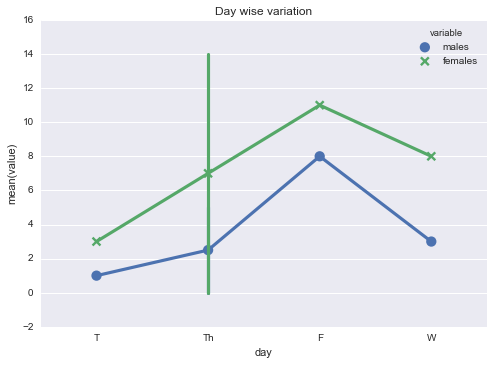
\includegraphics[width=\linewidth]{lineplot-daywise}
\end{figure}
\end{frame}


\begin{frame}[fragile]{Extras}
\begin{figure}
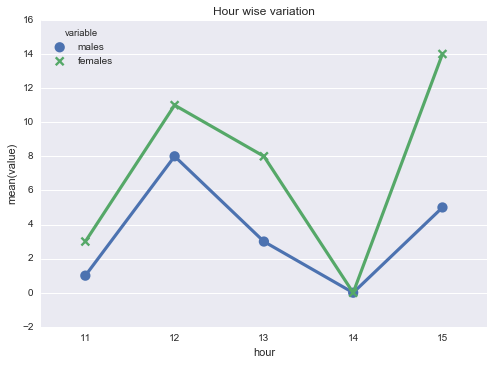
\includegraphics[width=\linewidth]{lineplot-hourwise}
\end{figure}
\end{frame}

\begin{frame}[fragile]{Extras}
\begin{figure}
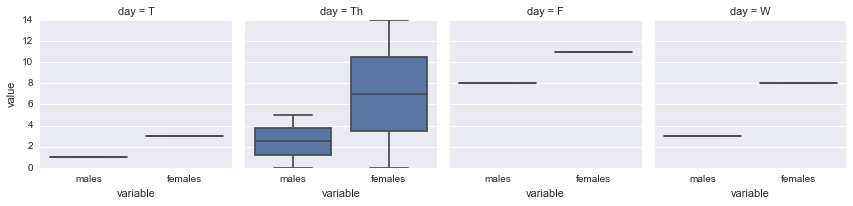
\includegraphics[width=\linewidth]{boxplots-daywise}
\caption{Boxplot}
\end{figure}
\end{frame}

\begin{frame}[fragile]{Next Week}
\begin{itemize}
\item Quiz![First five minutes!]. Based on lab sessions 01-02.
\item You don't need to know about things in 'Extras' slides
\item You should know about type of variables and should be able to determine them given a new experiment(Baking bread/Better fertilizer etc. that we talked about in Session 01) 
\item Please try to be on time!
\end{itemize}
\end{frame}

\begin{frame}[fragile]{Office Hours}
\Large \begin{center}Tuesday: 9-10AM\\
Thursday: 9-10AM\\
ZSH 372\\
\vspace*{2cm}
Saket Choudhary\\ 
skchoudh@usc.edu\\
\end{center}
\end{frame}

\end{document}
